\documentclass[11pt, sigconf]{acmart}
\usepackage{lipsum}
\usepackage{graphicx}
\usepackage[T1]{fontenc}
\usepackage{lmodern}
\begin{document}
\title{Recidivism Final Project Report}
\author{Andi Zhao, Helen Wu, Ryan Sun}
\date{\today}
\begin{abstract}
In a situation where algorithms dictate the future of humanity, one must proceed with extreme caution. For example, \emph{COMPAS}, a software that is employed by the legal system to predict the recidivism rate of criminals, came under fire for neglecting the aspect of fairness in 2016. The ProPublica organization discovered racial bias within the predicted results, indicating a lack of thought and consideration of ethics while creating the algorithm. Using a dataset from the Iowa state government correctional center website, our final project focuses on this subject matter by attempting to predict recidivism with and without eliminating protected features from the training set to see if it has any effect on predicting recidivism. Pre-processing was required to eliminate unnecessary features and missing information. This report will detail the process in which we gathered and processed the data, as well as the conclusions that we drew from comparing our different models. 
\end{abstract}
\settopmatter{printacmref=false}
\setcopyright{none}
\renewcommand\footnotetextcopyrightpermission[1]{}
\pagestyle{plain}
\maketitle

\section{Motivation and Objective}
\hspace{5mm}In recent years, the traditional justice system has been accused of being biased to minority populations. In an attempt to resolve this issue, researchers developed \emph{COMPAS} (Correctional Offender Management Profiling for Alternative Sanctions), a tool used to circumvent the need for human judgement. The reason that it came under fire was because it was yielding biased results where “blacks are almost twice as likely as whites to be labeled a higher risk but not actually re-offend”\cite{1}. In addition, privacy and fairness have been at the forefront of modern artificial intelligence research. Some researchers have attempted to train models without protected attributes to avoid lawsuits. We wondered if eliminating protected attributes from the training set actually has any effects on the accuracy and precision of the model. If the protected attribute has no effect on the accuracy of the model, it would mean that either race has no effect on the outcome of the model or that race was predicted. On the other hand, if race does have an effect, it would mean that the researchers were correct to hide the protected attribute. 


Our intention is to use Iowa’s recidivism dataset to train a model with and without race as one of its features to determine if race is a factor in determining recidivism. We also attempt to predict race from recidivism data to see whether or not the results are significant enough to associate race and recidivism. Our plan was to train two models, one with logistic regression and the other with decision trees, to compare accuracy, and other statistics. The goal of this project is to produce models that predict with similar accuracies to that of \emph{COMPAS}, as well as to uncover the relationship between using race as a feature and the corresponding results for predicting recidivism risk scores.

\section{Ethical Issues}

\hspace{5mm}The ProPublica study showcased the dangers of algorithmic decision making without concern for ethics, namely race, which can be detrimental to a true understanding and accurate modeling of recidivism. Additionally, the institutional biases within the \emph{COMPAS} algorithm directly affects our justice system because \emph{COMPAS} risk scores are actually considered by judges during sentencing in certain US states. The chart below shows the flaws and clear biases of blindly using the \emph{COMPAS} assessment to identify risk scores for an individual during sentencing.  
\begin{figure}[h] 	
\centering
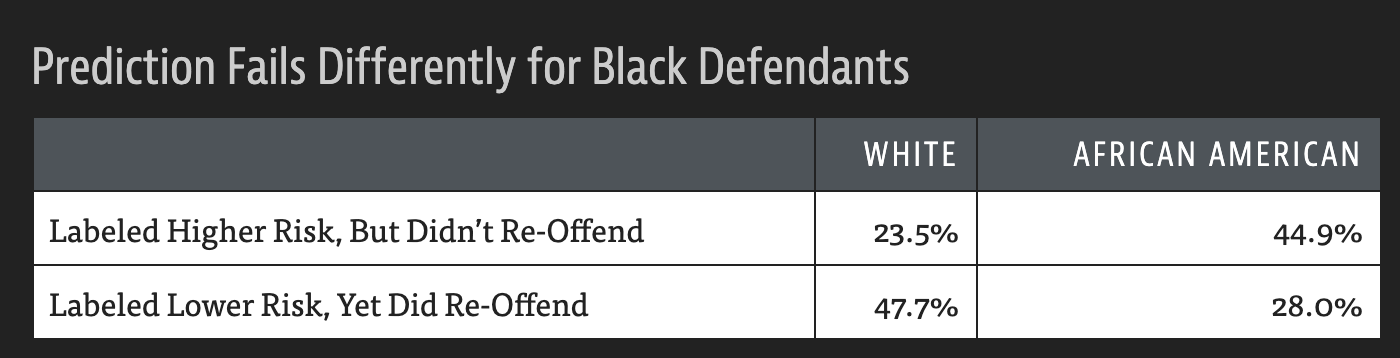
\includegraphics[width=3.3in]{asdf.png}
\caption{ProPublica's discovery}
\end{figure}


In our study, we are primarily concerned about whether or not using race as a feature will affect the prediction of recidivism for an individual. By including and excluding race as an attribute, we are able to create different models and compare their results, thus allowing us to determine whether or not race was a significant factor in the predictions. We also tried the opposite, using recidivism to predict race, to see if any ethical concerns arise. 


\section{Domain and Dataset}

\hspace{5mm}Initially, we wanted to use ProPublica's released data set as our main source of data. However, after analyzing the CSV file, we realized it was too convoluted to understand. Many of the column names were not self-explanatory and the documentation for each feature was lacking. Furthermore, there were duplicate information for some of the individuals, and cleaning and analyzing the data set would have taken far too long. After speaking to our TA about our project, we decided to utilize another data set released by Iowa state's government correctional center facility. Not only were these feature names straightforward and easy to understand, the data was cleaner and more recent. 

The data set contained recidivism information for 26,020 individuals from 2007-2013 in the state of Iowa. In total, there were 17 columns, with the "Return to Prison" column indicating whether the individual recidivated within the last 3 years. Out of the 17 attributes, age, race, and sex were the only 3 protected attributes in the data set. To protect the identities even further, each individuals age at release fell into a 5 categories; no actual ages were revealed. Strangely, the race category did not contain a unique Hispanic value as each of the other race groups were either Hispanic or Non-Hispanic (this can be seen in the graph below). This phenomenon in the data set is unusual as according to the 2010 US census, the Hispanic or Latino population was around 6\% of the total population, making it the second highest ethnic group population in the state.\cite{2}

After reviewing the data set, we decided to choose 5 non-protected attributes we thought were beneficial and relevant to creating our models. These 5 features were: Release Type, Age At Release, Offense Classification, Offense Type, and Target Population. Since we also wanted to test whether or not race affected the prediction results, we also added the race attribute as one of our features for two of our four models. While the former 5 features were relatively clean, the latter race feature was a little more difficult. Incomplete data (i.e., ‘White -’, ‘Black -’, ‘NA -’) littered the race column, and since we were not able to differentiate which group these incomplete values belonged to, we removed them from our data set. In addition, we replaced NaN with -1 and proceeded to remove any rows with missing values to avoid future complications of fitting models. This brought our total data set size down to 5,195.

Before we removed any rows, we wanted to see the original data set's ethnic group statistics and how it could impact our results. In Figure 2, the number of White and Non-Hispanics greatly outnumber the rest of the ethnicities. As we will see later, the heavily skewed data impacted the predictions of the four models we created. The chart below is a visual representation of the original dataset grouped by ethnicity and recidivism count. 

\begin{figure}[h] 	
\centering
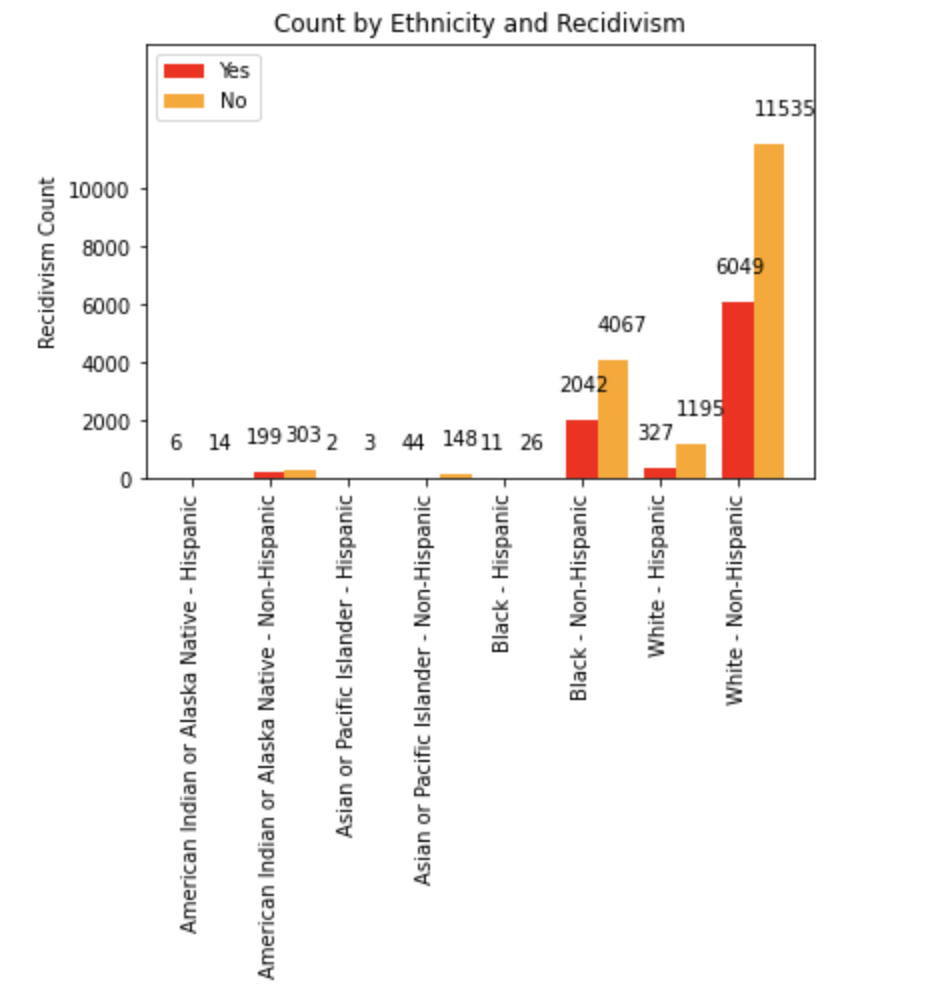
\includegraphics[width=3in]{1.png}
\caption{Data Distribution}
\end{figure}

\section{Models and Algorithms}
\subsection{Decision Trees}
\hspace{5mm} In this project, we primarily used sklearn’s decision tree as well as logistic regression packages to model the data. To keep things modularized, we created multiple models to predict both race and recidivism. When predicting for recidivism, we used both decision tree as well as logistic regression models to verify and compare the results. Models included and excluded race to check if race impacted recidivism predictions. When predicting for race, we used a decision tree with the recidivism feature.

In the decision tree models, a majority of the columns were binarized since many of the features that we selected for this project were mainly categorical features, such as ``Target Population" or ``Offense Classification". This required the transformation of each unique value of a categorical columns into separate 0-or-1 columns before being appended back into the dataset. The model that Included race as a feature would introduce many additional columns in the dataset, one for each unique value in the original column. After the transformation of the dataset into binarized values, the data is split into the testing and training sets before creating the model to predict for recidivism. To decide the depth parameter for the decision trees, we used accuracy as a measure of optimization for deciding the tree depth to use. 

In an attempt to predict race from recidivism features, the features that were previously removed from the data set were used. The new dataset with information about recidivism also had mostly categorical features, so the same process as before was repeated in order to binarize the features for a decision tree model. This model would predict on the 'Race' labels, and took the same approach as the decision tree models detailed above. 

\subsection{Logistic Regression}
$$TODO: Logreg$$




\section{Results and Analysis}
Results and Analysis – Report on the accuracy or any evaluation metric you used. You may use
plots, graphs and illustrations to describe your contributions.

To analyze the data of the decision trees, we chose to look at the accuracy, precision, and recall of the results. In the model predicting without race, we achieved an accuracy of 66.7\%, similar to that of COMPAS (63-67\% depending on race). The exact numbers our model had predicted was 213 cases of recidivism and 4982 non-recidivism cases. The labels for the testing data indicate 1729 cases of recidivism and 3466 non-recidivism cases. The next step was to create a model that predicted with race as a feature, and the results were similar: 225 predictions of ``Yes" for recidivism and 4970 predictions of ``No". The difference was ``only" a dozen more for ``Yes" when race was used as a feature to predict for recidivism. The charts below are the results graphed with matplotlib, and they are identical. 


\begin{figure}[h] 	
\centering
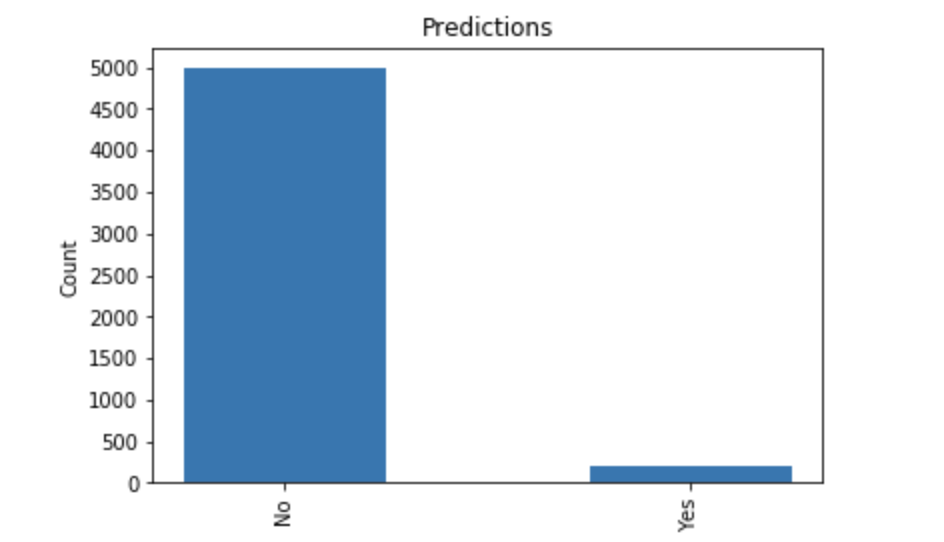
\includegraphics[width=3in]{2.png}
\caption{Without Race}
\end{figure}

\begin{figure}[h] 	
\centering
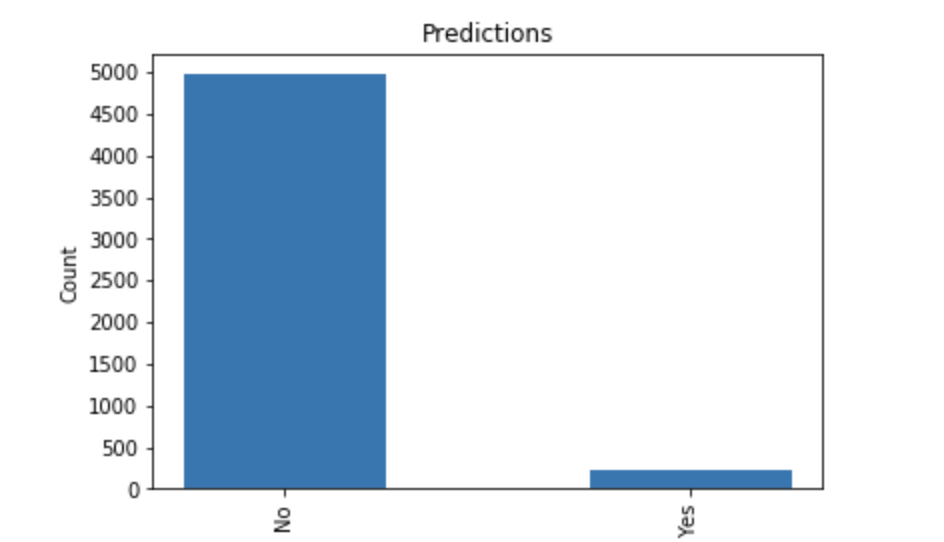
\includegraphics[width=3in]{3.png}
\caption{With Race}
\end{figure}

From a speculative standpoint, we thought that this could indicate that either race does not affect the outcome of the model, since the only difference in the models were the features they trained on, or that there could be some confounding variable present. 

The model that predicted race from recidivism features produced similarly skewed results. The model predicted the following:

\begin{tabular}{|c|c|c|}
\textbf{Race (Condensed)} & \textbf{Predictions} & \textbf{Actual} \\
 Indian  - Hispanic& 0 & 5 \\
Indian - Non-Hispanic& 0 & 94 \\
 Asian - Hispanic& 0 & 1\\
 Asian  - Non-Hispanic& 3 & 35\\
 Black - Hispanic&0 & 9 \\
 Black - Non-Hispanic& 75 &1244\\ 
 White - Hispanic& 23& 302 \\
 White - Non-Hispanic &5094&3505\\
\end{tabular}

\begin{figure}[h] 	
\centering
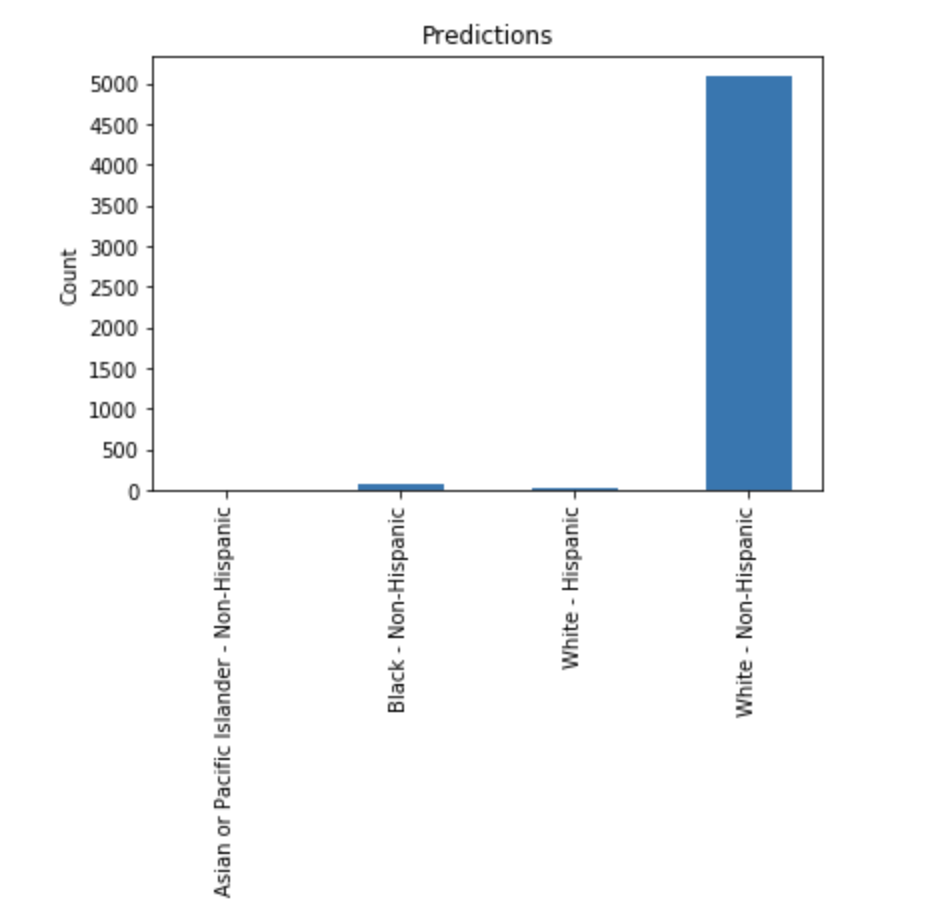
\includegraphics[width=3in]{4.png}
\caption{Predicting Race}
\end{figure}

Although skewed, this data still clocks in at 68\% accuracy, coincidentally similar to the accuracy of the model predicting recidivism. 
This model is predicting mainly 'White-Non-Hispanic' for almost every entry in the test data, with only around 100 predictions combined from the other ethnic groups. 

Perhaps optimizing the decision tree for accuracy may not have been the best choice, but it could also be simply due to the fact that our data represented the race groups differently as well. These decision tree results tell us that there are some intrinsic properties of this dataset that skews our results. Perhaps we need more features and data representing all ethnic groups equally to train and create a more accurate model. 

$$TODO: More~analysis $$

\section{Contribution}

\hspace{5mm}Ryan Sun created the decision tree models for predicting recidivism with and without race as a feature. He also created the model for predicting race from including recidivism features. Along with the group, he took part in the analysis of the results and created charts for the poster/video presentation. He also took part in authoring multiple sections of this report. 

Huanlei Wu did most of the pre-processing and pre-processing visualizations. At first, she considered adding neural networks and random forest classifiers as models, but ultimately decided against it. However, the code is still in the Jupyter notebook. She also helped Andi Zhao with some of the visualizations for the logistic regression model at the end of the project, mainly the two recidivism prediction graphs. In addition, she also took up the task of cleaning up and beautifying the group's code so it was more readable and easier to understand. Along with the whole group, she helped analyze the results, create the presentation poster, as well as write and proofread the final report. Her focus of the report was mainly on the "Domain and Dataset" portion. 

$$TODO: Andi~Zhao$$


\section{Future Work}

\hspace{5mm}An interesting follow-up for this project would to be create models for the original COMPAS dataset and compare the results to that of this project. Does the different in race representation between the large datasets in the data skew the results? Or are there further confounding factors present? Comparing the results to our current models could potentially provide further insight into the influence of race as a feature in machine learning models. 

Taking it a step further, we could also look at \emph{many} data sets and see how the protected attributes, especially race, affects recidivism predictions. We could look at more than just the basic measurable statistics of these results and explore many other possible connections as well. Further inquiries could possibly be made to pin down the true factor of race and ethnicity in these machine learning projects and algorithms. 



\begin{thebibliography}{1}

\bibitem{1}
Angwin, Julia; Larson, Jeff (2016-05-23). ``Machine Bias". ProPublica. Retrieved 2019-11-21.
\bibitem{2}
``U.S. Census Bureau QuickFacts: Iowa." Census Bureau QuickFacts, www.census.gov/quickfacts/-fact/table/
IA/POP010210.

\end{thebibliography}
\end{document}